
\documentclass[letterpaper, reqno,11pt]{article}
\usepackage[margin=1.0in]{geometry}
\usepackage{color,latexsym,amsmath,amssymb}
\usepackage{fancyhdr}
\usepackage{amsthm}
\usepackage[linesnumbered,lined,boxed,commentsnumbered,noend,noline]{algorithm2e}
\usepackage{dsfont}
\usepackage{graphicx}
\usepackage{hyperref}
\usepackage{bbm}
\usepackage[inline]{enumitem}
\usepackage[numbers]{natbib}
\usepackage{framed}
\usepackage{titling}
\usepackage{subcaption}
\usepackage[dvipsnames]{xcolor}
\usepackage{mathdots}
\usepackage{mathtools}
\usepackage{tikz}
\usetikzlibrary{hobby}
\usetikzlibrary{shapes.multipart}
\usetikzlibrary{intersections, calc}
\usepackage{pgfplots}
\pgfplotsset{compat=1.7}
\usetikzlibrary{arrows.meta}
\usetikzlibrary{decorations.markings}
\usetikzlibrary{shapes}
\usetikzlibrary{arrows}
\usepgfplotslibrary{fillbetween}
\usetikzlibrary{patterns}

\tikzset{invclip/.style={clip,insert path={{[reset cm]
  (-16383.99999pt,-16383.99999pt) rectangle (16383.99999pt,16383.99999pt)}}}}

\allowdisplaybreaks

\newcommand{\RR}{\mathbb{R}}
\newcommand{\CC}{\mathbb{C}}
\newcommand{\ZZ}{\mathbb{Z}}
\newcommand{\QQ}{\mathbb{Q}}
\newcommand{\NN}{\mathbb{N}}
\newcommand{\FF}{\mathbb{F}}
\newcommand{\PP}{\mathop{{}\mathbb{P}}}
\newcommand{\EE}{\mathop{{}\mathbb{E}}}
\newcommand{\LL}{\mathbb{L}}
\newcommand{\TT}{\mathbb{T}}
\newcommand{\GI}{\textrm{GI}}
\newcommand{\coGI}{\overline{\textrm{GI}}}
\DeclareMathOperator{\conv}{conv}
\DeclareMathOperator{\charcone}{char.cone}
\DeclareMathOperator{\STAB}{STAB}
\DeclareMathOperator{\Down}{Down}
\DeclareMathOperator{\lca}{lca}
\DeclareMathOperator{\ex}{ex}
\DeclareMathOperator{\Span}{span}
\DeclareMathOperator{\T}{\mathsf{T}}
\DeclareMathOperator{\F}{\mathsf{F}}
\DeclareMathOperator{\shP}{\# P}
\DeclareMathOperator{\shSAT}{\# SAT}
\DeclareMathOperator{\shDNF}{\# DNF}
\DeclareMathOperator{\DNF}{\mathsf{DNF}}
\DeclareMathOperator{\Poly}{\mathsf{P}}
\DeclareMathOperator{\CNF}{\mathsf{CNF}}
\DeclareMathOperator{\SAT}{\mathsf{SAT}}
\DeclareMathOperator{\BPP}{\mathsf{BPP}}
\DeclareMathOperator{\poly}{poly}
\DeclareMathOperator{\RP}{\mathsf{RP}}
\DeclareMathOperator{\EXP}{\mathsf{EXP}}
\DeclareMathOperator{\DTIME}{\mathsf{DTIME}}
\DeclareMathOperator{\NP}{\mathsf{NP}}
\DeclareMathOperator{\MCprime}{MC'}
\DeclareMathOperator{\Var}{Var}
\DeclareMathOperator{\IP}{\mathsf{IP}}
\DeclareMathOperator{\PSPACE}{\mathsf{PSPACE}}
\DeclareMathOperator{\lollipop}{lollipop}
\DeclareMathOperator{\ustconn}{\textsf{UST-Conn}}
\DeclareMathOperator{\RL}{\mathsf{RL}}
\DeclareMathOperator{\dist}{dist}
\DeclareMathOperator{\Ex}{Ex}
\DeclareMathOperator{\error}{error}
\DeclareMathOperator{\AND}{\mathsf{AND}}
\DeclareMathOperator{\ANDbar}{\mathsf{\overline{AND}}}
\DeclareMathOperator{\val}{val}
\DeclareMathOperator{\sign}{sign}
\DeclareMathOperator{\NS}{NS}
\DeclareMathOperator{\Maj}{Maj}
\DeclareMathOperator{\Inf}{Inf}
\DeclareMathOperator{\WL}{WL}
\DeclareMathOperator{\SL}{\textsc{StrongLearn}}
\DeclareMathOperator{\PCP}{\mathsf{PCP}}
\DeclareMathOperator{\threeSAT}{\mathsf{3SAT}}
\newcommand\mycommfont[1]{\ttfamily\textcolor{blue}{#1}}
\SetCommentSty{mycommfont}
\SetKwFor{RepTimes}{repeat}{times}{end}
\SetKw{Reject}{reject}
\SetKw{Accept}{accept}
\begin{document}
\pagenumbering{arabic}
\title{Lectures on Szemer\'edi's Regularity Lemma}
\author{Yuchong Pan}
\date{\today}
\newtheorem{theorem}{Theorem}
\newtheorem{lemma}[theorem]{Lemma}
\newtheorem{proposition}[theorem]{Proposition}
\newtheorem{corollary}[theorem]{Corollary}
\newtheorem{fact}[theorem]{Fact}
\newtheorem{problem}[theorem]{Problem}
\newtheorem{observation}[theorem]{Observation}
\newtheorem{claim}{Claim}
\newtheorem{exercise}{Exercise}
\theoremstyle{definition}
\newtheorem{definition}[theorem]{Definition}
%\maketitle
%

\begin{framed}
\noindent{\bf 6.842 Randomness and Computation} \hfill \thedate
\begin{center}
\Large{\thetitle}
\end{center}
\noindent{\em Lecturer: Ronitt Rubinfield} \hfill {\em Scribe: \theauthor}
\end{framed}

\section{Randomness and Regularity}

Random graphs have many nice properties, and various questions can be asked in a random graph. For instance, the following question asks for the expected number of triangles in a random tripartite graph:

\begin{problem}
  How many triangles are in a random tripartite graph with partition classes $A, B, C$ and density $\eta$?
\end{problem}

For all $u \in A, v \in B, w \in C$, let
$$ \sigma_{u, v, w} = \left\{
  \begin{array}{ll}
    1, & \text{if $u, v, w$ form a triangle}, \\
    0, & \text{otherwise}.
  \end{array}
\right. $$
Then for all $u \in A, v \in B, w \in C$,
$$ \EE\left[\sigma_{u, v, w}\right] = \PP\left[\sigma_{u, v, w} = 1\right] = \eta^3. $$
Hence,
$$ \EE[\text{\# triangles}] = \EE\left[\sum_{\substack{u \in A \\ v \in B \\ w \in C}} \sigma_{u, v, w}\right] = \eta^3 |A| |B| |C|. $$

Can we make a weaker assumption and still obtain reasonable bounds? In other words, what if the edges are not completely independent? We introduce the notions of \emph{desntity} and \emph{regularity} of set pairs to describe behaviors like those of a random graph.

\begin{definition}[density and regularity of set pairs]
  Let $G = (V, E)$ be a graph. Let $A, B \subset V$ be such that $A \cap B = \emptyset$ and $|A| > 1, |B| > 1$. Let $e(A, B)$ be the number of edges between $A$ and $B$. Let the \emph{density} of $(A, B)$ be defined to be $d(A, B) = e(A, B)/(|A| |B|)$. We say that $(A, B)$ is \emph{$\gamma$-regular} if for all $A' \subset A$ and $B' \subset B$ such that  $|A'| \geq \gamma |A|$ and $|B'| \geq \gamma |B|$,
  $$ \left|d\left(A', B'\right) - d(A, B)\right| < \gamma. $$
\end{definition}

In other words, the fraction of edges between $A'$ and $B'$ is roughly the same as the fraction of edges between $A$ and $B$.

\section{Triangle Counting Lemma}

In this example, we demonstrate the power of the notion of regularity of set pairs by proving the following lemma. Informally, we show that three disjoint subsets $A, B, C$ of vertices, each pair of which is $\gamma$-regular, contain many triangles. A random graph would have $\eta^3 |A||B||C|$ triangles, and $\gamma$-regular set pairs give $\eta^3/16 |A| |B| |C|$ triangles, which is only slightly worse within a constant factor than a random graph.

\begin{lemma}[triangle counting lemma] \label{lem:triangle-counting}
  Let $G = (V, E)$ be a graph. For all $\eta$ (called the \emph{density}), there exists $\gamma > 0$ (called the \emph{regularity parameter}) and $\delta > 0$ (the fraction of triangles) such that if $A, B, C$ are disjoint subsets of $V$ such that each pair is $\gamma$-regular with densities greater than $\eta$, then $G$ contains at least $\delta |A| |B| |C|$ distinct triangles with vertices in each of $A, B, C$.
\end{lemma}

We remark that $\gamma = \gamma^\triangle(\eta) := \eta/2$ and $\delta = \delta^\triangle(\eta) := (1 - \eta) \eta^3/8$ are functions of $\eta$ independent of the number of vertices or edges.

\begin{proof}
  Let $A^*$ be the vertices in $A$ with at least $|\eta - \gamma| |B|$ neighbors in $B$ and at least $|\eta - \gamma| |C|$ neighbors in $C$. We claim that $|A^*| \geq (1 - 2\gamma) |A|$. To see this, let $A'$ be the set of ``bad'' vertices with respect to $B$, i.e., with fewer than $|\eta - \gamma| |B|$ neighbors in $B$, and let $A''$ be the set of ``bad'' vertices in $C$, i.e., with fewer than $|\eta - \gamma| |C|$ neighbors in $C$. Then
  \begin{gather*}
    d\left(A', B\right) < \frac{\left|A'\right| \cdot |\eta - \gamma| \cdot |B|}{\left|A'\right| \cdot |B|} = |\eta - \gamma| = \eta - \gamma, \qquad d(A, B) = \eta.
  \end{gather*}
  It follows that the difference betweeen $d(A', B)$ and $d(A, B)$ is greater than $\gamma$. Since $B \geq \gamma |B|$ and since $(A, B)$ is $\gamma$-regular, then $|A'| < \gamma |A|$. Similarly, $|A''| < \gamma |A|$. Since $A^* = A \setminus (A' \cup A'')$, then
  $$ \left|A^*\right| \geq |A| - \left|A'\right| - \left|A''\right| \geq |A| - 2\gamma |A| = (1 - 2\gamma) |A|. $$

  For each $u \in A^*$, let $B_u$ be the set of neighbors of $u$ in $B$, and let $C_u$ be the set of neighbors of $u$ in $C$. Since $\gamma = \eta/2$, then $\eta - \gamma \geq \gamma$. Hence,
  \begin{align*}
    \left|B_u\right| &\geq |\eta - \gamma| |B| \geq \gamma |B|, \\
    \left|C_u\right| &\geq |\eta - \gamma| |C| \geq \gamma |C|.
  \end{align*}
  Note that the number of edges between $B_u$ and $C_u$ equals the number of triangles involving $u$. See Figure \ref{fig:triangle-counting} for an illustration.
  
  \begin{figure}[h]
    \centering
    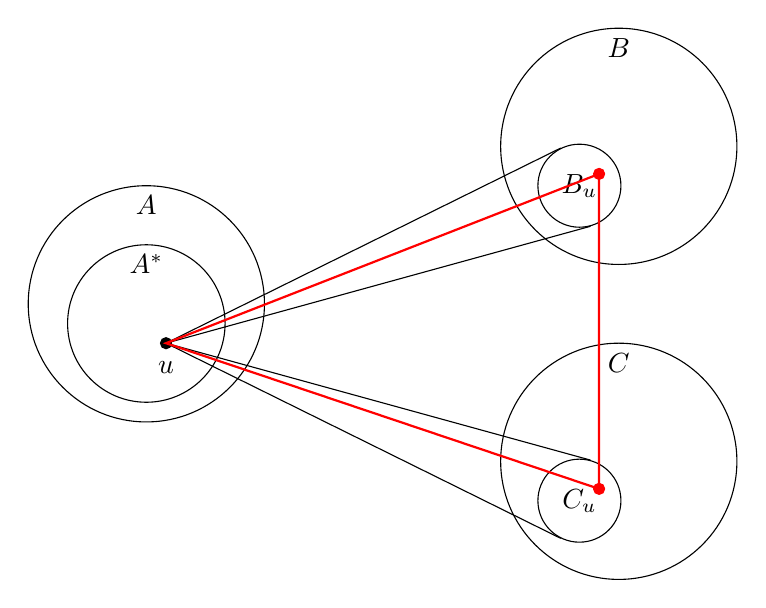
\begin{tikzpicture}
      \draw (0, 0) circle (1.5);
      \node at (0, 1.25) {$A$};
      \draw (0, -.25) circle (1);
      \node at (0, .5) {$A^*$};
      \draw (6, 2) circle (1.5);
      \node at (6, 3.25) {$B$};
      \draw (6, -2) circle (1.5);
      \node at (6, -.75) {$C$};
      \node [circle,draw,name path=circle] (bu) at (5.5, 1.5) [minimum size=30pt] {};
      \node at (5.5, 1.5) {$B_u$};
      \node [circle,draw,name path=circle] (cu) at (5.5, -2.5) [minimum size=30pt] {};
      \node at (5.5, -2.5) {$C_u$};
      \draw[fill=black] (.25, -.5) circle (2pt) node[below, yshift=-3pt] {$u$};
      \draw (.25, -.5)  -- (tangent cs:node=bu,point={(.25, -.5)},solution=1);
      \draw (.25, -.5)  -- (tangent cs:node=bu,point={(.25, -.5)},solution=2);
      \draw (.25, -.5)  -- (tangent cs:node=cu,point={(.25, -.5)},solution=1);
      \draw (.25, -.5)  -- (tangent cs:node=cu,point={(.25, -.5)},solution=2);
      \draw[red, fill=red] (5.75, 1.65) circle (2pt);
      \draw[red, fill=red] (5.75, -2.35) circle (2pt);
      \draw[red, thick] (.25, -.5) -- (5.75, 1.65) -- (5.75, -2.35) -- cycle;
    \end{tikzpicture}
    \caption{The number of edges between $B_u$ and $C_u$ equals the number of triangles involving $u$.}
    \label{fig:triangle-counting}
  \end{figure}
  
  Since $(B, C)$ is $\gamma$-regular, then $d(B_u, C_u) \geq \eta - \gamma$. Hence,
  $$ e\left(B_u, C_u\right) \geq (\eta - \gamma) \left|B_u\right| \left|C_u\right| \geq (\eta - \gamma) (\eta - \gamma) |B| (\eta - \gamma) |C| = (\eta - \gamma)^3 |B||C|. $$
  It follows that the total number of triangles is at least
  $$ \left|A^*\right| (\eta - \gamma)^3 |B||C| \geq (1 - 2\gamma) (\eta - \gamma)^3 |A||B||C| \geq (1 - \eta)\left(\frac{\eta}{2}\right)^3 |A||B||C| = \delta |A||B||C|. $$
  This completes the proof.
\end{proof}

\section{Szemer\'edi's Regularity Lemma}

Informally, Szemer\'edi's regularity lemma says that \emph{every} graph can be partitioned into a \emph{constant} number of $\gamma$-regular pairs. We state Szemer\'edi's regularity lemma without giving a proof due to time constraints.

\begin{theorem}[Szemer\'edi's regularity lemma]
  For all $m > 0$ and $\varepsilon > 0$, there exists $T = T(m, \varepsilon)$ such that for any graph $G = (V, E)$ with $|V| > T$ and any equi-partition $\mathcal A$ of $V$, there exists an equipartition $\mathcal B$ into $k$ sets which refines $\mathcal A$ such that $m \leq k \leq T$ and at most $\varepsilon \binom{k}{2}$ set pairs are not $\varepsilon$-regular.
\end{theorem}

Historically, Szemer\'edi's regularity lemma was first studied to prove a conjecture of Erd\H{o}s and Tur\'an that sequences of integers have long artihmetic progressions.

A very rough idea for the proof of Szemer\'edi's regularity lemma is as follows: We introduce the notion of the \emph{variance} of a partition of the vertices in a graph. Starting with an initial partition, whenever a partition violates regularity, we refine it such that the variance grows significantly, i.e., by approximately $\varepsilon^c$ for some constant $c$. Therefore, in fewer than $1/\varepsilon^c$ refinements, we have a good partition.

How big is $T$? The above construction shows that $T$ is in the order of
$$ \begin{rcases}
  2^{2^{\iddots^{\;2}}}
\end{rcases}\text{height $1/\varepsilon^c$}. $$
It is amazing that this is a constant independent of the number of vertices, although this is very large and not practical algorthmically.

\section{Triangle-Freeness Testing}

An application of Szemer\'edi's regularity lemma is triangle-freeness testing in a graph:

\begin{problem}[triangle-freeness testing]
  Let $G$ be a graph (not necessarily tripartite) and $\varepsilon > 0$. If $G$ is triangle-free, then accept. If one needs to delete at least $\varepsilon n^2$ edges to make $G$ triangle-free (i.e., $G$ is $\varepsilon$-far from being triangle-free), then reject.
\end{problem}

This model is interesting only in dense graph. We give an algorithm for triangle-free testing in Algorithm \ref{alg:triangle-free}.

\begin{algorithm}[h]
  \RepTimes{$O(1)$}{
    pick $v_1, v_2, v_3 \in V$ \\
    \If{$v_1, v_2, v_3$ form a triangle}{
      \Reject
    }
  }
  \Accept
  \caption{An algorithm for triangle-free testing in a graph $G = (V, E)$.}
  \label{alg:triangle-free}
\end{algorithm}

\begin{theorem}
  For all $\varepsilon > 0$, there exists $\delta > 0$ such that any graph $G = (V, E)$ $\varepsilon$-far from being triangle-free contains at least $\delta\binom{|V|}{3}$ distinct triangles.
\end{theorem}

\begin{proof}[Proof sketch]
  Apply Szemer\'edi's regularity lemma to $G$, obtaining an equi-partition of $V$ into $k$ sets, where $5/\varepsilon \leq k \leq T$ (i.e., $\varepsilon n/5 \geq n/k \geq n/T$). Let $\varepsilon' = \min(\varepsilon/5, \delta^\triangle(\varepsilon/5))$. Then at most $\varepsilon' \binom{k}{2}$ pairs of sets in the equi-partition are not $\varepsilon'$-regular. Delete edges that are
  \begin{enumerate}[label=(\roman*), itemsep=0pt]
    \item internal to the sets in the equi-partition;
    \item between non-regular pairs of sets in the equi-partition;
    \item between low-density (i.e., less than $\varepsilon/5$) pairs of sets in the equi-partition.
  \end{enumerate}
  We can show that we have deleted fewer than $\varepsilon n^2$ edges, so the resulting graph $G'$ contains at least one triangle. Moreover, any triangle in $G'$ satisfies the following:
  \begin{enumerate}[label=(\roman*), itemsep=0pt]
    \item the three vertices forming the triangle are in three distinct sets in the equi-partition;
    \item each pair of these three sets are regular;
    \item the density between each pair of these three sets is not low.
  \end{enumerate}
  Finally, applying the triangle counting lemma (i.e., Lemma \ref{lem:triangle-counting}) gives a lower bound on the number of distinct triangles in $G'$ and hence $G$, showing that indeed many triangles remain.
\end{proof}

\end{document}
